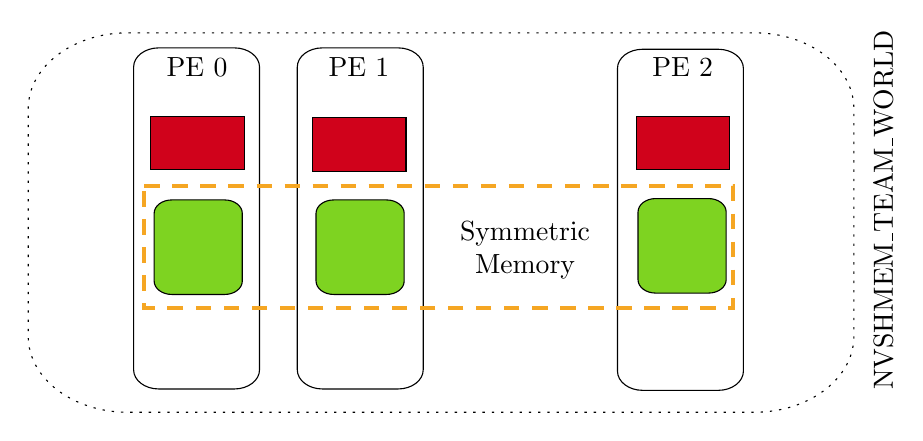
\begin{tikzpicture}[x=1pt,y=0.9pt,yscale=-0.55,xscale=0.65]
    %Rounded Rect [id:dp5682014849782169] 
    \draw   (100,34.25) .. controls (100,26.52) and (106.27,20.25) .. (114,20.25) -- (156,20.25) .. controls (163.73,20.25) and (170,26.52) .. (170,34.25) -- (170,255.25) .. controls (170,262.98) and (163.73,269.25) .. (156,269.25) -- (114,269.25) .. controls (106.27,269.25) and (100,262.98) .. (100,255.25) -- cycle ;
    %Rounded Rect [id:dp5262477048147362] 
    \draw   (191,34.25) .. controls (191,26.52) and (197.27,20.25) .. (205,20.25) -- (247,20.25) .. controls (254.73,20.25) and (261,26.52) .. (261,34.25) -- (261,255.25) .. controls (261,262.98) and (254.73,269.25) .. (247,269.25) -- (205,269.25) .. controls (197.27,269.25) and (191,262.98) .. (191,255.25) -- cycle ;
    %Rounded Rect [id:dp7573581856079369] 
    \draw   (369,35.25) .. controls (369,27.52) and (375.27,21.25) .. (383,21.25) -- (425,21.25) .. controls (432.73,21.25) and (439,27.52) .. (439,35.25) -- (439,256.25) .. controls (439,263.98) and (432.73,270.25) .. (425,270.25) -- (383,270.25) .. controls (375.27,270.25) and (369,263.98) .. (369,256.25) -- cycle ;
    %Shape: Rectangle [id:dp7570532028079713] 
    \draw  [fill={rgb, 255:red, 208; green, 2; blue, 27 }  ,fill opacity=1 ] (109.42,70.25) -- (161.42,70.25) -- (161.42,109.25) -- (109.42,109.25) -- cycle ;
    %Shape: Rectangle [id:dp19421520470566733] 
    \draw  [fill={rgb, 255:red, 208; green, 2; blue, 27 }  ,fill opacity=1 ] (199.42,71.25) -- (251.42,71.25) -- (251.42,110.25) -- (199.42,110.25) -- cycle ;
    %Shape: Rectangle [id:dp32300543498141965] 
    \draw  [fill={rgb, 255:red, 208; green, 2; blue, 27 }  ,fill opacity=1 ] (379.42,70.25) -- (431.42,70.25) -- (431.42,109.25) -- (379.42,109.25) -- cycle ;
    %Rounded Rect [id:dp6580910781722736] 
    \draw  [fill={rgb, 255:red, 126; green, 211; blue, 33 }  ,fill opacity=1 ] (111.42,141.05) .. controls (111.42,135.64) and (115.8,131.25) .. (121.22,131.25) -- (150.62,131.25) .. controls (156.03,131.25) and (160.42,135.64) .. (160.42,141.05) -- (160.42,190.45) .. controls (160.42,195.86) and (156.03,200.25) .. (150.62,200.25) -- (121.22,200.25) .. controls (115.8,200.25) and (111.42,195.86) .. (111.42,190.45) -- cycle ;
    %Rounded Rect [id:dp26363692092381197] 
    \draw  [fill={rgb, 255:red, 126; green, 211; blue, 33 }  ,fill opacity=1 ] (201.42,141.05) .. controls (201.42,135.64) and (205.8,131.25) .. (211.22,131.25) -- (240.62,131.25) .. controls (246.03,131.25) and (250.42,135.64) .. (250.42,141.05) -- (250.42,190.45) .. controls (250.42,195.86) and (246.03,200.25) .. (240.62,200.25) -- (211.22,200.25) .. controls (205.8,200.25) and (201.42,195.86) .. (201.42,190.45) -- cycle ;
    %Rounded Rect [id:dp18887280028716125] 
    \draw  [fill={rgb, 255:red, 126; green, 211; blue, 33 }  ,fill opacity=1 ] (380.42,140.05) .. controls (380.42,134.64) and (384.8,130.25) .. (390.22,130.25) -- (419.62,130.25) .. controls (425.03,130.25) and (429.42,134.64) .. (429.42,140.05) -- (429.42,189.45) .. controls (429.42,194.86) and (425.03,199.25) .. (419.62,199.25) -- (390.22,199.25) .. controls (384.8,199.25) and (380.42,194.86) .. (380.42,189.45) -- cycle ;
    %Rounded Rect [id:dp5265848887584798] 
    \draw  [color={rgb, 255:red, 0; green, 0; blue, 0 }  ,draw opacity=1 ][dash pattern={on 0.84pt off 2.51pt}] (41.42,64.65) .. controls (41.42,34.05) and (66.22,9.25) .. (96.82,9.25) -- (445.02,9.25) .. controls (475.61,9.25) and (500.42,34.05) .. (500.42,64.65) -- (500.42,230.85) .. controls (500.42,261.45) and (475.61,286.25) .. (445.02,286.25) -- (96.82,286.25) .. controls (66.22,286.25) and (41.42,261.45) .. (41.42,230.85) -- cycle ;
    %Shape: Rectangle [id:dp9039242900086101] 
    \draw  [color={rgb, 255:red, 245; green, 166; blue, 35 }  ,draw opacity=1 ][dash pattern={on 5.63pt off 4.5pt}][line width=1.5]  (106,121) -- (433.42,121) -- (433.42,210.25) -- (106,210.25) -- cycle ;
    
    % Text Node
    \draw (135.26,34.5) node   [align=left] {PE 0};
    % Text Node
    \draw (225.26,34.5) node   [align=left] {PE 1};
    % Text Node
    \draw (405.26,34.5) node   [align=left] {PE 2};
    % Text Node
    \draw (510,272) node [anchor=north west][inner sep=0.8pt]  [rotate=-270] [align=left] {NVSHMEM\_TEAM\_WORLD};
    % Text Node
    \draw (280,145) node [anchor=north west][inner sep=0.75pt]   [align=center] {Symmetric \\ Memory};
\end{tikzpicture}
